\subsection{Упражнение 1}

Что случится, если при увеличении std не менять M

\begin{lstlisting}[language=Python]
slider = widgets.IntSlider(min=2, max=100, value=11)
slider2 = widgets.FloatSlider(min=0, max=20, value=2)
interact(plot_filter, M=slider, std=slider2);
\end{lstlisting}

\begin{figure}[H]
	\begin{center}
		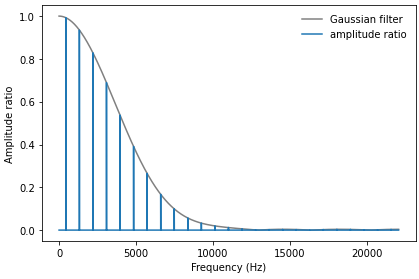
\includegraphics[scale=1]{fig/lab08/lab8_1.png}
		\caption{Гауссово окно для фильтрации}
	\end{center}
\end{figure}

\begin{lstlisting}[language=Python]
gaussian = scipy.signal.gaussian(M=11, std=11)
gaussian /= sum(gaussian)

plt.plot(gaussian, label='Gaussian')
decorate(xlabel='Index')
\end{lstlisting}
\begin{figure}[H]
	\begin{center}
		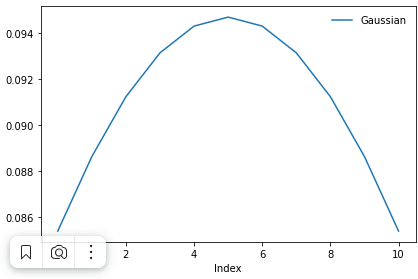
\includegraphics[scale=0.7]{fig/lab08/lab8_2.png}
		\caption{Гауссово окно}
	\end{center}
\end{figure}

\begin{lstlisting}[language=Python]
gaussian = scipy.signal.gaussian(M=11, std=1000)
gaussian /= sum(gaussian)

plt.plot(gaussian, label='Gaussian')
decorate(xlabel='Index')
\end{lstlisting}
\begin{figure}[H]
	\begin{center}
		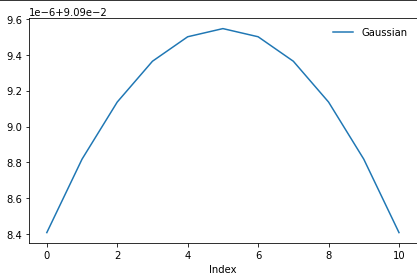
\includegraphics[scale=0.7]{fig/lab08/lab8_3.png}
		\caption{Гауссово окно}
	\end{center}
\end{figure}

Исходя из графиков видно, что БПФ стала меньше, а кривая - шире.

\subsection{Упражнение 2}

Выясним что происходит с преобразованием Фурье, если меняется std.

\begin{lstlisting}[language=Python]
gaussian = scipy.signal.gaussian(M=16, std=2)
gaussian /= sum(gaussian)

plt.plot(gaussian, label='Gaussian')
decorate(xlabel='Index')
\end{lstlisting}
\begin{figure}[H]
	\begin{center}
		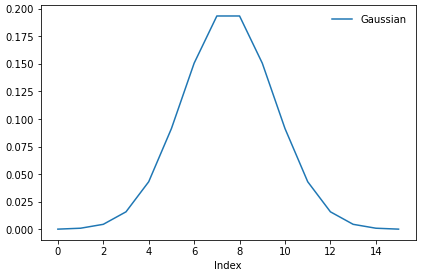
\includegraphics[scale=0.7]{fig/lab08/lab8_4.png}
		\caption{Гауссово окно}
	\end{center}
\end{figure}

\begin{lstlisting}[language=Python]
gaussian_fft = np.fft.fft(gaussian)
plt.plot(abs(gaussian_fft), label='Gaussian')
\end{lstlisting}
\begin{figure}[H]
	\begin{center}
		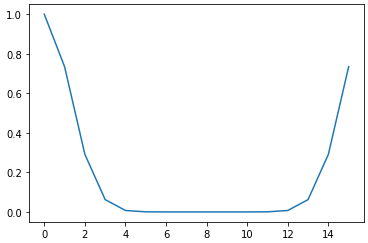
\includegraphics[scale=1]{fig/lab08/lab8_5.png}
		\caption{FTT применённое на окно}
	\end{center}
\end{figure}

Сделаем свертку отрицательных частот влево.

\begin{lstlisting}[language=Python]
gaussian_fft_rolled = np.roll(gaussian_fft, len(gaussian) // 2)
plt.plot(abs(gaussian_fft_rolled), label='Gaussian')
\end{lstlisting}
\begin{figure}[H]
	\begin{center}
		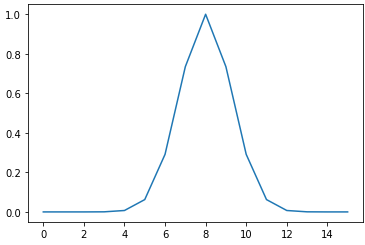
\includegraphics[scale=1]{fig/lab08/lab8_6.png}
		\caption{Результат свертки}
	\end{center}
\end{figure}

Можно отметить, что при увеличении std гауссовой кривой, преобразование Фурье становится уже.


\subsection{Упражнение 3}

Поработать с разными окнами. Какое из них лучше подходит для филтра НЧ?

Создадим сигнал длительностью равной 1 секунде и протестируем.

\begin{lstlisting}[language=Python]
import thinkdsp
sig = thinkdsp.TriangleSignal(freq=440)
wave = sig.make_wave(duration=1.0, framerate=44100)
wave.make_audio()
\end{lstlisting}

\begin{lstlisting}[language=Python]
sig.plot()
\end{lstlisting}

\begin{figure}[H]
	\begin{center}
		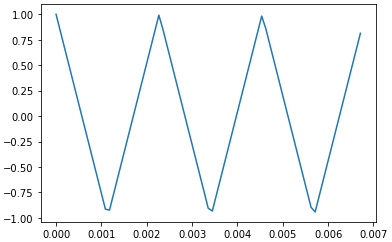
\includegraphics[scale=1]{fig/lab08/lab8_7.png}
		\caption{Пилообразный сигнал}
	\end{center}
\end{figure}

Далее создадим различные окна


\begin{lstlisting}[language=Python]
M = 16
std = 2

g = scipy.signal.gaussian(M,std)
br = np.bartlett(M)
bl = np.blackman(M)
hm = np.hamming(M)
hn = np.hanning(M)

array  = [gaussian,bartlett,blackman,hamming,hanning]
labels = ['gauss','barlett','blackman','hamming','hanning']

for elem, label in zip(array,labels):
  elem /= sum(elem)
  plt.plot(elem,label=label)
plt.legend()
\end{lstlisting}

\begin{figure}[H]
	\begin{center}
		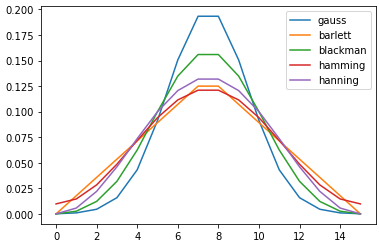
\includegraphics[scale=1]{fig/lab08/lab8_8.png}
		\caption{Применение различных окон на выбранный сигнал}
	\end{center}
\end{figure}

Дополним окна нулями и выведем ДПФ:

\begin{lstlisting}[language=Python]
for elem, label in zip(array, labels):
  padded =  zero_pad(elem, len(wave))
  dft_window = np.fft.rfft(padded)
  plt.plot(abs(dft_window), label=label)
plt.legend()
\end{lstlisting}
\begin{figure}[H]
	\begin{center}
		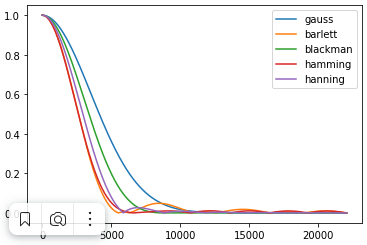
\includegraphics[scale=1]{fig/lab08/lab8_9.png}
		\caption{Применение различных окон на выбранный сигнал}
	\end{center}
\end{figure}

Изменим маштаб.

\begin{lstlisting}[language=Python]
for elem, label in zip(array, labels):
  padded =  zero_pad(elem, len(wave))
  dft_window = np.fft.rfft(padded)
  plt.plot(abs(dft_window), label=label)
plt.legend()
decorate(yscale='log')
\end{lstlisting}
\begin{figure}[H]
	\begin{center}
		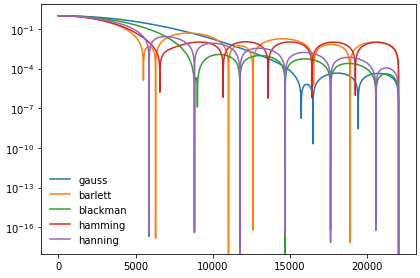
\includegraphics[scale=1]{fig/lab08/lab8_10.png}
		\caption{Логорифмический масштаб}
	\end{center}
\end{figure}

Исходя из результатов можно предположить, что Хэнинг лучше всего подходит для фильтрации низких частот.

\subsection{Вывод}

В ходе данной ЛР были рассмотренны операции фильтрации, сглаживания и свертки. Каждая из этих операций может быть полезной для какой-либо определенной задачи. Например, сглаживание удаляет быстрые изменения сигнала для выявления общих особенностей.
